\documentclass[10pt,landscape,a4paper]{article}
\usepackage[utf8]{inputenc}
\usepackage[ngerman]{babel}
\usepackage[T1]{fontenc}
\usepackage{adigraph}
\usepackage{tikz}
\usetikzlibrary{shapes,positioning,arrows,fit,calc,graphs,graphs.standard}
\usepackage[nosf]{kpfonts}
\usepackage[t1]{sourcesanspro}
\usepackage{multicol}
\usepackage{wrapfig}
\usepackage[top=1mm,bottom=2mm,left=2mm,right=2mm]{geometry}
\usepackage[framemethod=tikz]{mdframed}
\usepackage{microtype}
\usepackage{pdfpages}
\usepackage{xfrac}
\usepackage{tikz-cd}
\usepackage{pgfplots}
\pgfplotsset{compat = newest}
\usepackage{graphicx}
\graphicspath{ {./img/} }

\let\bar\overline

\begin{document}


\include{inhalt/def}

\small
\begin{multicols*}{3}

\section{Funktionen}
\subsection{Symetrien}
\begin{itemize}
    \item Eine Funktion $f$ heisst gerade, wenn $f(-x) = f(x)$ für alle $x \in D$.\\\\
    \begin{tikzpicture}[scale=0.7]
        \begin{axis}[
            axis lines = middle,
            xlabel = $x$,
            ylabel = $y$,
            enlargelimits]
            \addplot[domain = -10:10,
            samples = 200,
            smooth,
            thick,
            blue] {x^2};
        \end{axis}
    \end{tikzpicture}
    \item Eine Funktion $f$ heisst ungerade, wenn $f(-x) = -f(x)$ für alle $x \in D$.\\\\
    \begin{tikzpicture}[scale=0.7]
        \begin{axis}[
            axis lines = middle,
            xlabel = $x$,
            ylabel = $y$,
            enlargelimits]
            \addplot[domain = -10:10,
            samples = 200,
            smooth,
            thick,
            blue] {x^3};
        \end{axis}
    \end{tikzpicture}
\end{itemize}
\subsection{Umkehrfunktionen}
Für die Umkehrfunktionen einfach nach x auflösen und dann x und y vertauschen.\\
Eigenschaften von Umkehrfunktionen:
\begin{itemize}
    \item Für jede Relation R gilt $R^{-1^{-1}} = R$
    \item R ist genau dann linksvollständig, wenn $R^{-1}$ rechtseindeutig ist.
    \item R ist genau dann linkseindeutig, wenn $R^{-1}$ rechtseindeutig ist.
\end{itemize}
\subsection{Komposition}
Für $g: A \rightarrow B $ und $f: B \rightarrow C$ definieren wir:
\begin{align*}
    f \circ g: A \rightarrow C
\end{align*}
\begin{align*}
    (f \circ g)(x) = f(g(x))
\end{align*}
Wörtlich sagt man auch ''f nach g'' da f nach g ausgeführt wird bzw. g zuerst ausgeführt wird.
\subsubsection{Assoziativität}
Für $f: A \rightarrow B$, $g: B \rightarrow C$ und $h: C \rightarrow D$ gilt:
\begin{itemize}
    \item $(f \circ g) \circ h = f \circ (g \circ h)$
\end{itemize}
\subsection{Summenformel}
Arithmetische Summenformel:
\begin{align*}
    \sum_{i=1}^{n} i = \frac{n(n+1)}{2}
\end{align*}
Summe der Quadratzahlen:
\begin{align*}
    \sum_{i=1}^{n} i^2 = \frac{n(n+1)(2n+1)}{6}
\end{align*}
\subsection{Betragsfunktion}
\begin{center}
\begin{tikzpicture}[scale=0.7]
    \begin{axis}[
        axis lines = middle,
        xlabel = $x$,
        ylabel = $y$,
        enlargelimits]
        \addplot[domain = -10:10,
        samples = 200,
        smooth,
        thick,
        blue] {abs(x)};
    \end{axis}
\end{tikzpicture}
\end{center}
\begin{align*}
    |x| = \begin{cases}
        x & \text{für } x \geq 0\\
        -x & \text{für } x < 0
    \end{cases}
\end{align*}
\section{Polynome}
\subsection{Definition}
Ein Polynom ist eine Funktion der Form:
\begin{align*}
    p(x) = a_n x^n + a_{n-1} x^{n-1} + \ldots + a_1 x + a_0
\end{align*}
\subsection{Nullstellen}
Im Polynom $f(x) = (x-1)(x+3)(x-8)^2(x-6)^3$ ist 8 eine Doppelnullstelle und 6 eine Dreifachnullstelle.\\
\subsubsection{Nullstellen Raten}
In Analyis 1 der ZHAW dürfen zudem Nullstellen geraten werden. Diese sind immer im folgenden Bereich: $\{-3,-2,-1,0,1,2,3\}$
\subsection{Horner-Schema}
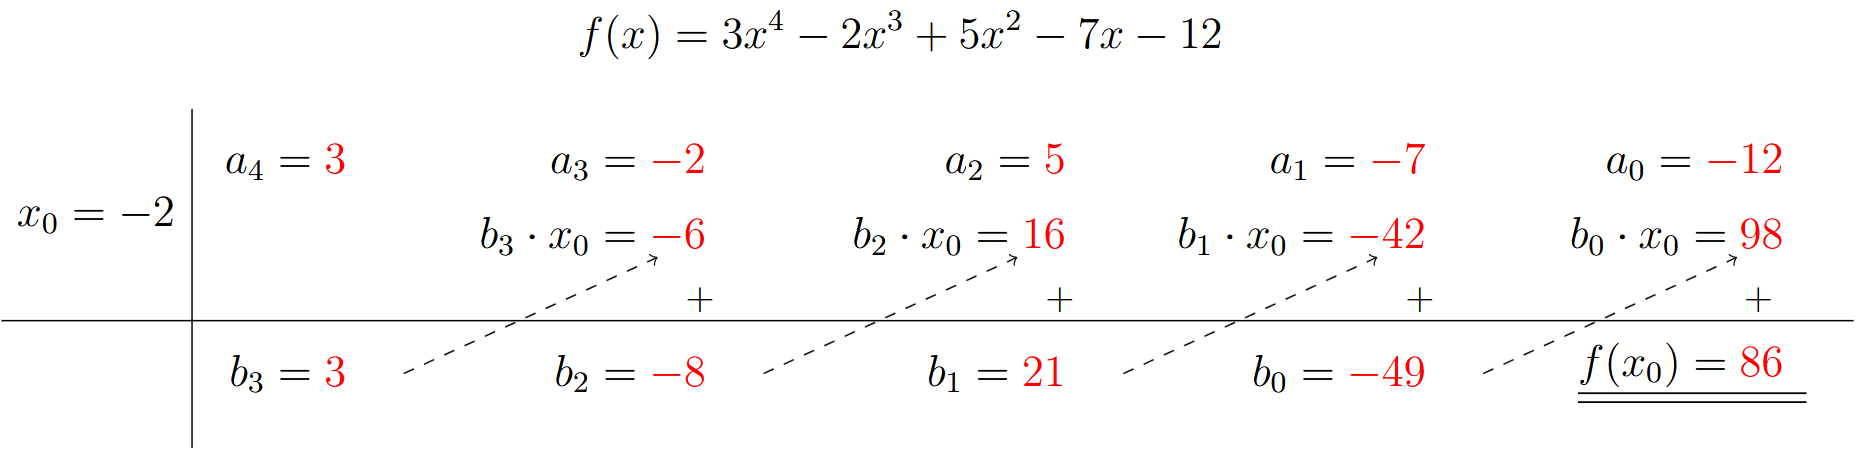
\includegraphics[scale=0.2]{horner}
\subsection{Polynomdivision}
\begin{center}
    \textbf{GOOD LUCK HOMIE}
\end{center}
\section{Ableiten}
\subsection{Ableitungsregeln}
\subsubsection{Faktorregel}
\begin{align*}
    (c \cdot f)(x)' = c \cdot f'(x)
\end{align*}
\subsubsection{Summenregel}
\begin{align*}
    (f+ g)(x)' = f'(x) + g'(x)
\end{align*}
\subsubsection{Produktregel}
\begin{align*}
    (u \cdot v)'(x) = u'(x) \cdot v(x) + u(x) \cdot v'(x)
\end{align*}
\subsubsection{Quotientenregel}
\begin{align*}
    \left(\frac{u}{v}\right)'(x) = \frac{u'(x) \cdot v(x) - u(x) \cdot v'(x)}{(v(x))^2}
\end{align*}
\subsubsection{Kettenregel}
\begin{align*}
    (F \circ u)'(x) = F'(u) \cdot u'(x)
\end{align*}
\subsection{Ableitungen bestimmter Funktionen}
\begin{itemize}
    \item $sin(x)' = cos(x)$
    \item $cos(x)' = -sin(x)$
    \item $(e^x)' = e^x$
    \item $(e^{-20x})' = -3 \cdot e^{-3x}$
    \item $(a^x)' = a^x \cdot ln(a)$
    \item $(ln(x))' = \frac{1}{x}$
    \item $(log_a(x))' = \frac{1}{x \cdot ln(a)}$
\end{itemize}
\subsection{Linearisierung einer Funktion}
Die Funktionsgleichung für die Tangente von $f(x)$ an der Stelle $x_0$ lautet:
\begin{align*}
    y = f'(x_0) \cdot (x - x_0) + f(x_0)
\end{align*}
\subsection{Newton-Verfahren}
\begin{align*}
    x_{n+1} = x_n - \frac{f(x_n)}{f'(x_n)}
\end{align*}
\section{Integral}
Um die Fläche unter einer Funktion zu berechnen muss man folgende Schritte durchgehen:
\begin{enumerate}
    \item Bestimme die Stammfunktion $F(x)$
    \item Berechne $F(b) - F(a)$
\end{enumerate}
\subsection{Stammfunktion}
Die Stammfunktion $F(x)$ einer Funktion $f(x)$ ist die Funktion, deren Ableitung $f(x)$ ist, also "aufleiten".
\subsection{Satz}
Gegeben ist eine Funktion $f$, die auf einem Intervall $I$ stetig ist, und eine beliebige Stamm-
funktion $F$ von $f$. Dann gilt für alle $a, b \in I$:
\begin{align*}
    \int_a^b f(x)\,dx = F(b) - F(a)
\end{align*}
\subsection{Integrale von bestimmten Funktionen}
\subsubsection{Potenz- und Logharithmusfunktionen}
\begin{itemize}
    \item $\int a^x dx = \frac{a^x}{ln(a) + C}$
    \item $\int ln(x) dx = x \cdot ln(x) - x + C$
    \item $\int log_a(x) dx = \frac{1}{ln(a)} \cdot (x \cdot ln(x) -x) + C$
\end{itemize}
\subsubsection{Trigonometrische Funktionen}
\begin{itemize}
    \item $\int \sin(x) \, dx = -\cos(x) + C$
    \item $\int \cos(x) \, dx = \sin(x) + C$
    \item $\int \tan(x) \, dx = -\ln|\cos(x)| + C$
    \item $\int (1 + \tan^2(x)) \, dx = \int \frac{1}{\cos^2(x)} \, dx = \tan(x) + C$
    \item $\int (1 - x^2)^{-1/2} \, dx = \arcsin(x) + C$
    \item $\int -(1 - x^2)^{-1/2} \, dx = \arccos(x) + C$
    \item $\int (1 + x^2)^{-1} \, dx = \arctan(x) + C$
\end{itemize}
\section{Folgen und Reihen}
\subsection{Folgen}

\subsubsection{Grenzwert von Folgen}
\textbf{Fall 1}: Zählergrad < Nennergrad. Dann gilt:
\begin{align*}
	\lim_{n \to \infty} \frac{g(n)}{h(n)} & = 0
\end{align*}
\begin{align*}
	\textcolor{red}{\lim_{n \to \infty} \frac{3n^2 + 7n - 15}{n^3 - 2n^2 + n + 10} = 0}
\end{align*}
\textbf{Fall 2}: Zählergrad > Nennergrad. Dann gilt:
\begin{align*}
	\lim_{n \to \infty} \frac{g(n)}{h(n)} & = \infty \text{ oder } -\infty
\end{align*}
\begin{align*}
	\textcolor{red}{\lim_{n \to \infty} \frac{3n^4 + 7n - 15}{6n^3 - 2n^2 + 10} \to \infty}
\end{align*}
\textbf{Fall 3}: Zählergrad = Nennergrad. Dann gilt:
\begin{align*}
	\lim_{n \to \infty} \frac{g(n)}{h(n)} & = \frac{\text{führender Term von } g}{\text{führender Term von } h}
\end{align*}
\begin{align*}
	\textcolor{red}{\lim_{n \to \infty} \frac{2n^3 + n^2 + 8n}{5n^3 + 4n^2 + 17} = \frac{2}{5}}
\end{align*}
\textbf{Spezialfall}: Folge führt gegen $e \approx 2.718$:
\begin{align*}
	\lim_{n \to \infty} (1+\frac{1}{n})^n & = e
\end{align*}
\begin{align*}
	\textcolor{red}{\left(1 + \frac{k}{n}\right)^{n/m} = \left(1 + \frac{k}{n}\right)^{\frac{n}{k} \cdot \frac{k}{n} \cdot \frac{n}{m}} = \left(\left(1 + \frac{k}{n}\right)^{\frac{n}{k}}\right)^{\frac{\cancel{n}k}{\cancel{n}m}} \cdot \frac{\cancel{n}}{\cancel{n}} = \left(\left(1 + \frac{k}{n}\right)^{\frac{n}{k}}\right)^{\frac{k}{m}} = e^{\frac{k}{m}}}
\end{align*}

\subsection{Rechnen mit Grenzwerten}
\begin{align*}
	\lim_{n \to \infty} c \cdot a_n & = c \cdot \lim_{n \to \infty} a_n
\end{align*}
\begin{align*}
	\lim_{n \to \infty} (a_n + b_n) & = \lim_{n \to \infty} a_n + \lim_{n \to \infty} b_n
\end{align*}
\begin{align*}
	\lim_{n \to \infty} (a_n \cdot b_n) & = \lim_{n \to \infty} a_n \cdot \lim_{n \to \infty} b_n
\end{align*}
\begin{align*}
	\lim_{n \to \infty}(\frac{a_n}{b_n}) & = \frac{\lim_{n \to \infty} a_n}{\lim_{n \to \infty} b_n}
\end{align*}
\subsubsection{Arithmetische Reihe}
\begin{align*}
	a_k & = a_1 + (k-1) \cdot d
\end{align*}
\begin{align*}
    s_n & =n \cdot a_1 + \frac{n \cdot (n-1)}{2} \cdot d
\end{align*}
\begin{itemize}
	\item $s_n$ = Summe der ersten n Glieder
	\item $a_1$ = Erstes Glied
	\item $a_n$ = n-tes Glied
	\item $d$ = Differenz
\end{itemize}
\subsubsection{Geometrische Reihe}
\begin{align*}
    s_n & = a_1 \cdot \frac{q^n-1}{q-1}
\end{align*}
\begin{align*}
	a_n & = a_1 \cdot q^{n-1}
\end{align*}
\begin{itemize}
	\item $s_n$ = Summe der ersten n Glieder
	\item $a_1$ = Erstes Glied
	\item $a_n$ = n-tes Glied
	\item $q$ = Quotient
\end{itemize}
\subsubsection{Explizit und Implizit}
\begin{itemize}
	\item \textbf{Explizit}: $a_n = a_1 \cdot q^{n-1}$
	\item \textbf{Implizit}: $a_{3} = a_2 + x$
\end{itemize}

\subsubsection{$q$ herausfinden}
In einer Geometrischen Folge ist gegeben: $a_3 = 12$ und $a_5 = 20$\\
\begin{align*}
	q_2 & = \frac{a_5}{a_3}\\
	q & = (\frac{a_5}{a_3})^{\frac{1}{2}}
\end{align*}


\subsubsection{Grenzwert von Reihen}
\textbf{Arithmetische Reihe}\\
Geht (divergiert) immer gegen $\infty$ oder $-\infty$
\\
\\
\textbf{Geometrische Reihe}\\
Eine geometrische Reihe konvergiert genau dann, wenn $|q| < 1$ ist.
\begin{flushleft}
    \textit{\textbf{Fall 1}}: $q > 1$ \\
    Die Reihe strebt gegen $\infty$ oder $-\infty$. \\[0.5em]
    \textit{\textbf{Fall 2}}: $q \leq -1$ \\
    Die Reihe springt zwischen positiven und negativen Werten hin und her. \\[0.5em]
    \textit{\textbf{Fall 3}}: $|q| < 1$ \\
    Die Reihe strebt gegen $\frac{a_1}{1-q}$.
\end{flushleft}

\section{Grenzwert von Funktionen}
$\lim_{x \to x_0}f(x) = g$ bedeutet, dass $f(x)$ für $x_0$ gegen $g$ geht.\\
z.B. ist $\lim_{x \to 2} x^2 = 4$, da $x^2$ an der Stelle $2$, genau den Wert $4$ hat.\\
\subsection{Rechnen mit Grenzwerten}
\begin{align*}
    \lim_{x \to x_0}(c \cdot f(x)) & = c \cdot (\lim_{x \to x_0} f(x))
\end{align*}
\begin{align*}
    \lim_{x \to x_0}(f(x) + g(x)) & = \lim_{x \to x_0} f(x) + \lim_{x \to x_0} g(x)
\end{align*}
\begin{align*}
    \lim_{x \to x_0}(f(x) \cdot g(x)) & = (\lim_{x \to x_0} f(x)) \cdot (\lim_{x \to x_0} g(x))
\end{align*}
\begin{align*}
    \lim_{x \to x_0}\frac{f(x)}{g(x)} & = \frac{\lim_{x \to x_0} f(x)}{\lim_{x \to x_0} g(x)}
\end{align*}
\subsection{Gebrochenrationale Funktionen}
\subsubsection{Hebbare Definitionslücke}
Zählerpolynom und Nennerpolynom haben \textbf{beide} eine Nullstelle. Durch kürzen kann die Definitionslücke
aufgehoben werden.
\begin{align*}
    \textcolor{red}{f(x) = \frac{x^2-1}{x-1} = \frac{(x+1)(x-1)}{x-1} = x+1}
\end{align*}
\begin{align*}
    \textcolor{red}{\lim_{x \to 1} f(x) = 2}
\end{align*}
\begin{center}
\begin{tikzpicture}[scale=0.7]
    \begin{axis}[
        axis lines = middle,
        xlabel = $x$,
        ylabel = $y$,
        enlargelimits,
        xmin = -2, xmax = 4,
        ymin = -2, ymax = 4]
        \addplot[domain = -2:4,
        samples = 200,
        smooth,
        thick,
        blue] {(x^2)-1)/(x-1)}; 
        \addplot[only marks, mark=*, mark options={scale=1.5, fill=white}] coordinates {(1,2)};
    \end{axis}
\end{tikzpicture}
\end{center}
\subsubsection{Polstelle}
Wenn \textbf{nur} das Nennerpolynom eine Nullstelle (nach Kürzen) hat, dann hat die Funktion eine Polstelle.
\begin{center}
    \begin{tikzpicture}[scale=0.7]
        \begin{axis}[
            axis lines = middle,
            xlabel = $x$,
            ylabel = $y$,
            xmin = -1, xmax = 6,
            ymin = -1, ymax = 10]
            \addplot[domain = -10:10,
            samples = 200,
            smooth,
            thick,
            blue] {1/((x-2)^2)};
        \end{axis}
    \end{tikzpicture}
\end{center}
\subsection{Grenzwert von Funktionen in $\infty$}
Der Grenzwert $g$ einer Funktion $f$ für $x \to \infty$ bezeichnet den Wert, der die Funktion annimmt, 
wenn $x$ gegen unendlich geht.
\subsection{Stetigkeit von Funktionen}
Eine Funktion $f(x)$ heisst \textbf{stetig} an der Stelle $x_0$, wenn der Grenzwert von 
$\lim_{x \to x_0} f(x)$ existiert und $= f(x_0)$ ist. Vereinfacht, eine Funktion ist auf einem Intervall 
$I$ stetig, wenn sich ihr Graph in einem Zug, ohne Absetzen, zeichnen lässt.
\subsubsection{Stetigkeits-Aufgaben}
\begin{enumerate}
    \item Prüfen welche Schritte machen (muss ich noch Ableiten für z.B. Differenzierbarkeit?)
    \item Gleichungen für $f_1(1) = f_2(1)$, $f_2(2) = f_3(2)$... usw. aufstellen.
    \item Nach Unbekannter auflösen.
\end{enumerate}
\subsubsection{Einschachteln von Nullstelle}
Falls eine Funktion $f(x)$ auf einem Intervall $[a, b]$ stetig ist, und $f(a)$ und $f(b)$ verschiedene
Vorzeichen haben, dann hat $f$ in $[a, b]$ mindestens eine Nullstelle.
\section{Kurvendiskussion}
\subsection{Wendepunkte und Sattelpunkte}
\begin{align*}
	f''(x_0) = 0 \text{ und } f'''(x_0) \neq 0 \Rightarrow \textbf{Wendepunkt}
\end{align*}
\begin{align*}
	f'(x_0) = 0 \text{ und } f''(x_0) = 0 \text{ und } f'''(x_0) = 0 \Rightarrow \textbf{Sattelpunkt}
\end{align*}
\subsection{Monotonie}
Mithilfe dieses Satzes lassen sich monotone Abschnitte von Funktionen bestimmen:
\begin{align*}
	f'(x) & \text{ ist auf einem Intervall überall } \geq 0 \Leftrightarrow f \text{ ist auf diesem Intervall monoton steigend.} \\
	f'(x) & \text{ ist auf einem Intervall überall } \leq 0 \Leftrightarrow f \text{ ist auf diesem Intervall monoton fallend.}
\end{align*}
\subsection{Fragenkatalog}
\begin{enumerate}
	\item Defnitionsbereich?
	\item Symmetrieeigenschaften (gerade/ungerade), Periode?
	\item Schnittpunkte mit Achsen, Polstellen?
	\item Randpunkte bzw. Verhalten, wenn $x$ gegen die Grenzen des Defnitionsbereichs strebt?
	\item Kandidaten für Extrema bestimmen und untersuchen
	\item Wendepunkte suchen
	\item Tabelle von Werten aufstellen (falls noch nötig)
\end{enumerate}
\subsection{Extremwertaufgaben}
Siehe Kurvendiskussion für Maxima und Minima.\\
\begin{enumerate}
	\item Zielgrösse identifizieren.
	\item Unabhängige Variable identifizieren.
	\item Definitionsbereich bestimmen.
	\item Zielgrösse als Funktion der unabhängigen Variablen ausdrücken; ev. eine qualitative Skizze des Graphen machen.
	\item Relative Maxima resp. Minima bestimmen; Randpunkte auch berücksichtigen!
	\item Untersuchen, welche der relativen Extrema auch absolute Extrema sind (inklusive bei offenen und halboffenen Intervallen – Betrachtung der Funktion in der Nähe des Randes)
	\item Die gesuchte Information aus den Berechnungen extrahieren. (Ev. nachschauen, nach welcher Grösse gefragt wurde: Extremalstelle? Extremalwert? Extremalpunkt?)
\end{enumerate}

\end{multicols*}
\end{document}